\section{Diagrammi di sequenza}

\subsection{Notifica nuovo PDF caricato nella classe}
Come si può vedere in figura \ref{fig:seq_pdf}, quando un insegnante carica un nuovo PDF all'interno di una classe, se lo studente ha attivato le notifiche per quella classe, riceverà una notifica. Questo processo parte direttamente dal server che, previa registrazione dell'utente per le notifiche e richiesta del consenso, invia la notifica al dispositivo dell'utente tramite il servizio di notifiche push.\\
Nel diagramma è omessa la parte relativa alla richiesta del consenso e della registrazione per semplicità, ma è comunque un passaggio fondamentale per poter ricevere le notifiche.
\begin{figure}[h!]
    \centering
    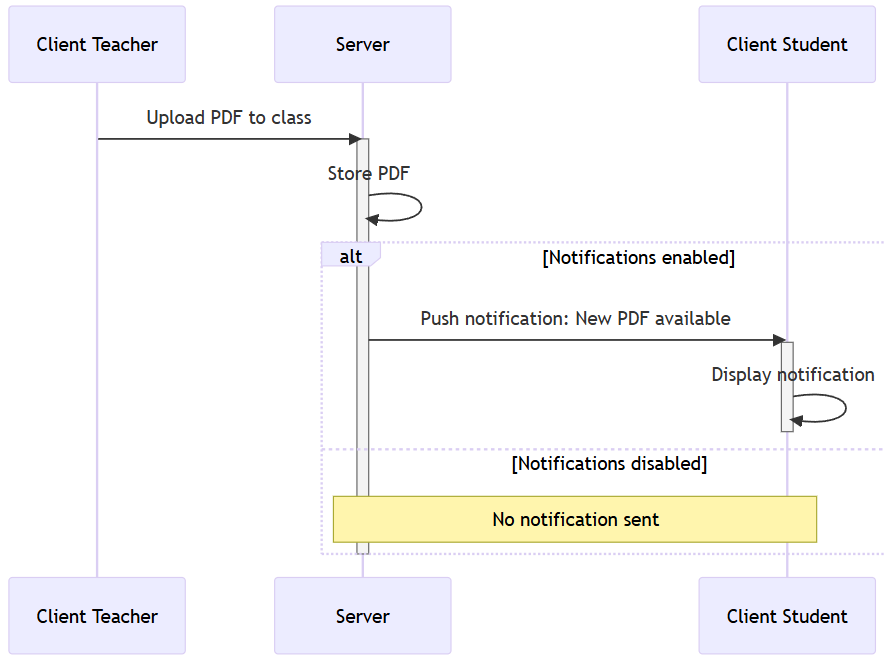
\includegraphics[width=1\textwidth]{diagrams/Sequence-pdf.png}
    \caption{Diagramma di sequenza per la notifica relativa ad un nuovo PDF}
    \label{fig:seq_pdf}
\end{figure}